\documentclass[a4paper,10pt]{article}
\usepackage{lineno}
\usepackage{graphicx}
\usepackage{amsmath}
\usepackage{amsthm}
\usepackage{amsfonts}
\usepackage{amssymb}% Required for inserting images
\newtheorem{lemma}{Lemma}
\newtheorem{proposition}{Proposition}
\usepackage{cite}
\usepackage{pgfplots}
\usepgfplotslibrary{groupplots}
\pgfplotsset{compat=1.18}
\usepackage{float}
\usepackage[utf8]{inputenc}             % UTF-8 编码
\usepackage[T1]{fontenc}                % 正确的字体编码
\usepackage{lmodern}                    % 现代字体
\usepackage{geometry}                   % 页面设置，可选
\geometry{margin=0.5in}   \usepackage{subcaption}  % 推荐 modern package
\usetikzlibrary{calc,3d,arrows,decorations.pathreplacing,patterns,positioning,backgrounds,shapes,intersections,matrix}
\usepackage{booktabs}
\usepackage{xcolor}
\usepackage{colortbl} 
\usepackage{diagbox}


% 绘图核心包（基础图形、流程、示意图依赖）
\usepackage{bm}                           % 粗体向量 \bm{v}
\usepackage{mathtools}                    % AMS math 的增强版


\usepackage{tikz}
\usetikzlibrary{%
  arrows,          % 箭头
  calc,            % 坐标计算
  3d,              % 3D 坐标
  shapes,          % 图形形状
  positioning,     % 相对位置
  backgrounds,     % 背景层
  decorations.pathreplacing, % 花括号装饰线
  patterns,        % 填充图案
  intersections,   % 线段交点
  matrix           % 矩阵布局
}


% 数据可视化包（曲线、柱状、3D、极坐标图依赖）

\usepackage{pgfplots}

% 固定PGFPlots版本兼容性（避免不同版本语法冲突，建议使用1.18及以上）

\pgfplotsset{compat=1.18}

% 加载TikZ扩展库（图案、箭头、几何形状、阴影、背景、定位）

\usetikzlibrary{patterns, arrows.meta, shapes.geometric, shadows, backgrounds, positioning}
% 核心配色：RGB值已转换为LaTeX支持的0-1范围（避免颜色显示异常）

\definecolor{nature-blue}{RGB}{0, 114, 178}    % 主蓝色（实验组、关键元素）

\definecolor{nature-red}{RGB}{213, 94, 0}      % 橙红色（对照组、警示元素）

\definecolor{nature-green}{RGB}{0, 158, 115}   % 绿色（处理组、正向元素）

\definecolor{nature-yellow}{RGB}{240, 228, 66} % 黄色（辅助元素、高亮）

\definecolor{nature-purple}{RGB}{204, 121, 167}% 紫色（特殊流程、次要元素）

\definecolor{nature-gray}{RGB}{86, 86, 86}     % 深灰色（网格、边框、文字）

% 淡色系列（流程图背景、辅助区域）

\definecolor{light-blue}{RGB}{230, 240, 250}   % 淡蓝色

\definecolor{light-red}{RGB}{255, 235, 220}    % 淡橙色

\definecolor{light-green}{RGB}{220, 245, 235}  % 淡绿色

% Portable fallback used because algorithm2e is not available in the current
% TeX installation. It preserves the two pseudocode blocks as numbered
% figures and implements the subset of algorithm2e commands used below.
\newenvironment{algorithm}[1][]{%
  \begin{figure}[H]\small\hrule\medskip
  \renewcommand{\;}{\par}%
}{%
  \medskip\hrule\end{figure}%
}
\newcommand{\SetAlgoLined}{}
\newcommand{\SetKwInOut}[2]{}
\newcommand{\Input}[1]{\textbf{Input:} #1\par}
\newcommand{\Output}[1]{\textbf{Output:} #1\par}
\newcommand{\KwIn}[1]{\textbf{Input:} #1\par}
\newcommand{\KwOut}[1]{\textbf{Output:} #1\par}
\newcommand{\BlankLine}{\medskip}
\long\def\ForEach#1#2{%
  \par\textbf{for each }#1\textbf{ do}\par
  \begingroup\leftskip=1.5em #2\par\endgroup}
\long\def\If#1#2{%
  \par\textbf{if }#1\textbf{ then}\par
  \begingroup\leftskip=1.5em #2\par\endgroup}
\long\def\Else#1{%
  \par\textbf{else}\par
  \begingroup\leftskip=1.5em #1\par\endgroup}
\newcommand{\Return}[1]{\par\textbf{return }#1\par}
\newcommand{\safeincludegraphics}[2][]{%
  \IfFileExists{#2}{%
    \includegraphics[#1]{#2}%
  }{%
    \fbox{\parbox[c][3.2cm][c]{0.92\linewidth}{%
      \centering Missing figure file\\[0.4em]\texttt{#2}}}%
  }%
}

\newcommand{\printbibliography}{%
  \bibliographystyle{unsrt}%
  \bibliography{ref}%
}

\begin{document}
\linenumbers
\title{A Treecode-based Algorithm with Locally Refined Meshes for
Hartree Potential Evaluation in Electronic Structure
Calculations}
\author{huan xiao}
\date{February 2026}


\maketitle

\tableofcontents


\section*{Abstract}

Efficient and reliable evaluation of the Hartree potential is essential in large-scale electronic structure simulations. Treecode methods provide a promising way to reduce the computational complexity of the Coulomb interaction, while adaptive finite element discretizations offer significant savings in degrees of freedom through local mesh refinement. However, combining these two techniques is nontrivial: the hierarchical structure required by tree-based acceleration may conflict with the irregular geometry and locality of adaptively refined meshes, making it difficult to construct efficient interaction lists and maintain computational efficiency.

To address this challenge, we develop a treecode algorithm within the adaptive finite element framework AFEPack. Two key components are introduced to ensure both efficiency and accuracy. First, a geometry-based mesh preprocessing strategy is designed to reorganize adaptive elements according to their spatial relationships and refinement hierarchy, enabling a consistent interaction structure compatible with treecode evaluation. Second, a multipole acceptance criterion (MAC) based on explicit error estimates is employed to control the approximation error and balance near-field and far-field interactions.

With these components, far-field interactions are approximated using multipole
expansions, while near-field contributions are computed directly, resulting in
an efficient matrix-free algorithm for adaptive meshes.

ke y words
\section{Introduction}

Electronic structure calculations play a central role in understanding the physical and chemical properties of atoms, molecules, and solids. Among various quantum mechanical approaches, density functional theory (DFT) has become one of the most widely used methods due to its favorable balance between computational efficiency and predictive accuracy
\cite{Hohenberg1964,Kohn1965,Parr1989,Martin2004,Jones2015}.
Based on the Hohenberg--Kohn theorems and the Kohn--Sham formulation, the many-electron problem is transformed into a set of effective single-particle equations, whose solution provides the ground-state electron density and related physical quantities
\cite{Hohenberg1964,Kohn1965}.

In atomic units, the stationary Kohn--Sham equations can be written as the nonlinear eigenvalue problem
\begin{equation}
\label{eq:kohn_sham}
\left[-\frac{1}{2}\nabla^2
+V_{\mathrm{eff}}[\rho](\mathbf r)\right]
\psi_i(\mathbf r)
=\varepsilon_i\psi_i(\mathbf r),
\qquad i=1,\ldots,N_{\mathrm{orb}},
\end{equation}
subject to the orthonormality conditions
\begin{equation}
\int_{\mathbb R^3}
\psi_i^*(\mathbf r)\psi_j(\mathbf r)\,d\mathbf r
=\delta_{ij}.
\end{equation}
The electron density and the effective potential are given by
\begin{equation}
\label{eq:ks_density_potential}
\rho(\mathbf r)
=\sum_{i=1}^{N_{\mathrm{orb}}}f_i|\psi_i(\mathbf r)|^2,
\qquad
V_{\mathrm{eff}}[\rho]
=V_{\mathrm{ext}}+V_H[\rho]+V_{\mathrm{xc}}[\rho],
\end{equation}
where \(f_i\) is the occupation number of the \(i\)th orbital and
\(\sum_i f_i=N_e\). Here \(V_{\mathrm{ext}}\) is the external potential
generated by the nuclei, \(V_H\) is the Hartree potential, and
\(V_{\mathrm{xc}}\) is the exchange--correlation potential. Since both
\(V_H\) and \(V_{\mathrm{xc}}\) depend on \(\rho\),
Eqs.~\eqref{eq:kohn_sham}--\eqref{eq:ks_density_potential} are solved
self-consistently.

In real-space Kohn--Sham density functional theory, finite element methods (FEM) have been developed as a flexible alternative to traditional basis-set approaches, providing geometric adaptability, systematic approximation control, and applicability to complex electronic systems. However, electronic wave functions and charge densities often exhibit strong spatial variations near nuclei, chemical bonds, and localized states, making uniform discretizations computationally inefficient. To overcome this limitation, adaptive finite element methods (AFEM) have been introduced, where a posteriori error estimators are employed to identify regions requiring higher resolution and guide local mesh refinement. Recent developments by Hu, Yang, and collaborators have established adaptive finite element frameworks for Kohn--Sham equations by combining multilevel correction techniques with adaptive refinement strategies, enabling efficient large-scale real-space electronic structure simulations
\cite{BaoHuLiu2012,HuXieXu2018,YangShenHu2021}. These adaptive approaches naturally generate hierarchical and highly nonuniform meshes, which provide an efficient representation of electronic densities while introducing new computational challenges for evaluating long-range interactions.

Spatial adaptivity addresses only one source of cost in a Kohn--Sham calculation. At every self-consistent-field (SCF) step, the occupied eigenspace must also be updated for a large, changing Hamiltonian. Preconditioned block eigensolvers such as LOBPCG provide an effective alternative to full diagonalization \cite{Knyazev2001}, whereas Chebyshev-filtered subspace iteration reuses the occupied subspace from the preceding SCF step and replaces repeated eigensolutions by polynomial filtering and a reduced Rayleigh--Ritz calculation \cite{ZhouSaad2006}. Complementary reductions in computational cost have been obtained through adaptive local basis functions in a discontinuous Galerkin formulation \cite{LinLuYingE2012}. At the software level, higher-order adaptive spectral finite elements, Chebyshev filtering, domain decomposition, and band parallelism have been combined in DFT-FE for large-scale Kohn--Sham calculations \cite{Motamarri2020}; its subsequent hybrid CPU--GPU implementation accelerates the principal computational kernels \cite{Das2022}. These developments show that a scalable real-space solver requires efficient algorithms not only for the Kohn--Sham eigenproblem, but also for the repeated construction of the electrostatic potential.

The Hartree potential is a fundamental component of Kohn--Sham density functional theory
\cite{Kohn1965,Parr1989,Martin2004}, describing the classical electron--electron interaction generated by the charge density. For a given electronic density $\rho(\mathbf r)$, it is defined by the Coulomb integral
\[
V_H(\mathbf r)=
\int_{\mathbb{R}^{3}}
\frac{\rho(\mathbf r')}
{|\mathbf r-\mathbf r'|}
\,d\mathbf r'.
\]
Due to the long-range behavior and singularity of the Coulomb kernel, the efficient and accurate evaluation of the Hartree potential remains a major computational bottleneck in real-space electronic structure simulations, particularly when adaptive finite element discretizations are employed.

The Hartree potential can alternatively be obtained by solving the equivalent Poisson equation
\[
-\nabla^2 V_H = 4\pi\rho,
\]
because the Coulomb kernel $1/|\mathbf r-\mathbf r'|$ is the Green's function of the Laplace operator in $\mathbb{R}^3$. Although the Poisson formulation avoids direct evaluation of the singular integral, it requires assembling and solving a globally coupled stiffness matrix
\cite{Hackbusch1985,Saad2003}. With mesh refinement, the condition number typically increases as $\mathcal{O}(h^{-2})$, leading to increased computational cost and stronger dependence on effective preconditioners. Furthermore, elliptic solvers involve global coupling, communication, and coarse-grid operations, which may introduce additional challenges for large-scale parallel implementations.

An alternative strategy is to directly evaluate the Coulomb integral. However, discretization of the integral formulation leads to dense pairwise interactions between source and target degrees of freedom, resulting in a computational complexity of $\mathcal{O}(N^2)$ for direct evaluation. This high computational cost has motivated the development of various fast algorithms for long-range interactions in electronic structure calculations and related applications.

Fast Fourier transform (FFT)-based approaches accelerate Coulomb interactions by exploiting convolution structures and have been widely used in plane-wave-based electronic structure methods. For isolated systems, free-space Poisson solvers based on interpolating scaling functions and FFT convolution can attain high accuracy with $\mathcal{O}(N\log N)$ work \cite{Genovese2006}. Their efficiency, however, relies on structured Cartesian grids and uniform sampling, making their direct application to highly adaptive finite element meshes nontrivial. Hierarchical methods, including the fast multipole method (FMM)
\cite{Greengard1987}
and treecode algorithms
\cite{Barnes1986,Appel1985},
provide an alternative framework by exploiting the spatial locality of long-range interactions. These methods recursively partition the computational domain into hierarchical clusters and approximate the collective contribution of distant source regions through multipole expansions. Consequently, the computational complexity can be reduced from $\mathcal{O}(N^2)$ to nearly linear or $\mathcal{O}(N\log N)$ while maintaining controllable approximation accuracy.

Among hierarchical fast summation methods, treecode algorithms provide several advantages for adaptive finite element discretizations. Unlike FFT-based methods, treecodes do not require structured grids and can naturally handle irregular spatial distributions. Compared with FMM, treecodes employ a simpler target-centered traversal strategy and avoid additional hierarchical translation operations, making them attractive for integration with adaptive mesh frameworks. Moreover, the inherent near-field/far-field decomposition of treecodes is well suited for adaptive meshes, where interactions in locally refined regions can be evaluated directly while well-separated regions are accelerated through multipole approximations. The accuracy and efficiency of a treecode depend strongly on its multipole acceptance criterion and traversal strategy \cite{Salmon1994,Dehnen2000}. More recently, treecode formulations have been developed for Poisson problems on general domains with unstructured grids \cite{Cui}, including a $p$-adaptive variant that selects expansion orders according to local error requirements \cite{CuiYang2025}. Therefore, treecode provides an effective approach for accelerating Hartree potential evaluation on highly nonuniform finite element meshes while preserving scalability.

However, the application of tree-based fast summation methods to adaptive finite element discretizations remains challenging. In FEM, source distributions are represented over mesh elements rather than point particles, and the computational mesh is generated through adaptive refinement driven by a posteriori error estimation
\cite{Verfurth1996,Binev2004}. Such meshes exhibit strong spatial nonuniformity and multiscale structures, with a hierarchy intrinsically associated with the finite element discretization. Conventional tree construction techniques, which are typically designed for particle systems or uniform grids, may introduce additional geometric preprocessing costs or fail to preserve the locality information contained in the adaptive mesh. Furthermore, classical multipole acceptance criteria (MACs) generally rely only on geometric separation and do not explicitly exploit the element-wise structure and refinement hierarchy of adaptive finite element meshes. Developing an interaction hierarchy that simultaneously preserves mesh locality, computational efficiency, and approximation accuracy therefore remains a key challenge.

In this work, we develop a geometry-based treecode framework that directly exploits the refinement hierarchy of adaptive finite element meshes. In contrast to constructing an independent spatial tree for an already discretized source distribution, the existing adaptive mesh hierarchy is employed as the backbone of the interaction tree. Consequently, clustering and interaction classification are naturally inherited from the geometric refinement process, avoiding redundant tree construction while preserving the locality of the finite element discretization. Within this framework, near-field interactions are evaluated accurately through elementwise numerical integration, while far-field contributions are accelerated using truncated multipole expansions
\cite{Greengard1987}. An error-based multipole acceptance criterion is incorporated to control truncation errors and improve robustness
\cite{Barnes1986}. By integrating the discretization hierarchy and interaction hierarchy into a unified framework, the proposed method provides a consistent coupling between adaptive finite element discretizations and treecode acceleration. Under standard assumptions on hierarchical refinement and interaction admissibility, the preprocessing and traversal procedures retain the expected $\mathcal{O}(N\log N)$ complexity of treecode algorithms even for highly nonuniform adaptive meshes.

The proposed method is implemented within the adaptive finite element framework \textsc{AFEPack}
\cite{AFEPack}. The resulting algorithm is matrix-free and parallel-friendly, avoiding the assembly and solution of globally coupled linear systems. By combining adaptive finite element discretization with geometry-consistent treecode acceleration, the proposed approach provides an efficient and scalable framework for Hartree potential evaluation in large-scale real-space Kohn--Sham DFT simulations.

article construction

\section{review}
\label{sec:motivation}

\subsection{Hartree potential evaluation on a locally refined mesh}

In a real-space electronic-structure calculation, the Hartree potential
must be reevaluated as the electron density changes.  On a locally refined
mesh, this operation must retain high resolution near localized features
without allowing the long-range Coulomb interaction to restore the cost of
a globally fine discretization.  Let \(\mathcal T_h\) denote the set of
\(n\) active tetrahedral leaves and let \(\rho\) be the density on the
truncated domain \(\Omega\).  The potential at a target point
\(\mathbf r\) is
\[
V_H(\mathbf r)
=
\int_{\Omega}
\frac{\rho(\mathbf r')}
{\vert \mathbf r - \mathbf r' \vert}
\, d\mathbf r'.
\]
Elementwise evaluation gives
\[
V_H(\mathbf r_i)
=
\sum_{K\in\mathcal T_h}
\int_K
\frac{\rho(\mathbf r')}{|\mathbf r_i-\mathbf r'|}
\,d\mathbf r'.
\]
With one representative target per active leaf, direct evaluation couples
\(n\) targets to \(n\) source elements and therefore has quadratic
interaction cost before accounting for the quadrature points within each
element.  In addition, the singular target element requires different
treatment from smooth distant contributions.  These features motivate a
geometric separation of nearby and distant interactions.

For hierarchical acceleration, the domain is partitioned into source
regions $\{\Omega_j\}_{j=1}^{N_c}$, where $N_c$ is the number of source
clusters.  The potential can then be written as
\[
V_H(\mathbf r)
=
\sum_{j=1}^{N_c}
\int_{\Omega_j}
\frac{\rho(\mathbf r')}
{\vert \mathbf r - \mathbf r' \vert}
\, d\mathbf r'.
\]

In the treecode framework,
the interaction between the target point $\mathbf r$
and a source cluster $\Omega_j$
is classified as either near-field or far-field
through a multipole acceptance criterion (MAC).
Let $\mathbf c_j$ denote the center of cluster $\Omega_j$,
$R_j$ its characteristic radius,
and $d_j = |\mathbf r - \mathbf c_j|$
the distance between the target point
and the cluster center.
The cluster is regarded as well separated if
\[
\frac{R_j}{d_j} < \theta,
\]
where $\theta \in (0,1)$
is a user-defined admissibility parameter.
If the MAC condition is not satisfied,
the interaction is treated as near-field
and evaluated directly through numerical integration.
Otherwise,
the contribution from the entire cluster
is approximated collectively
using a truncated multipole expansion about $\mathbf c_j$.

Accordingly,
the Hartree potential is decomposed into
\[
V_H(\mathbf r)
=
V_{\mathrm{near}}(\mathbf r)
+
V_{\mathrm{far}}(\mathbf r),
\]
where $V_{\mathrm{near}}$
contains directly evaluated nearby interactions,
while $V_{\mathrm{far}}$
contains far-field multipole approximations.
By replacing a large number of direct interactions
with hierarchical cluster approximations,
the overall computational complexity
is reduced from $\mathcal{O}(N^2)$
to nearly $\mathcal{O}(N\log N)$.
\subsection{Limitations of conventional treecodes on locally refined meshes(\color{red}figure)}

Tree-based fast summation techniques have been successfully
extended from particle systems to grid-based discretizations,
particularly on uniform or quasi-uniform meshes.
In such settings, the computational domain can be partitioned
into a hierarchy of regular cells, forming a well-structured tree.

For example, Cui et al.~\cite{Cui} developed a treecode algorithm
for evaluating long-range potentials on uniform meshes.
In their approach, the domain is recursively subdivided into
regular cells, and interactions are organized through a standard
tree traversal procedure.
Near-field interactions are evaluated directly on grid elements,
while far-field contributions are approximated using multipole
expansions associated with cell clusters.

The effectiveness of this approach relies on several key properties
of uniform meshes.
First, the tree structure is naturally balanced, since all cells
at the same level have comparable sizes.
Second, the geometric relation between clusters is consistent
throughout the domain, allowing a simple multipole acceptance
criterion (MAC), such as the size-distance ratio, to reliably
classify interactions.
As a result, both the computational efficiency and the accuracy
of the method can be maintained in a straightforward manner.

However, these properties depend critically on the assumption
of geometric regularity.
When the mesh becomes locally refined, as in adaptive finite
element discretizations, this assumption no longer holds.

In adaptive meshes, element sizes may vary by several orders
of magnitude, and the distribution of degrees of freedom
becomes highly nonuniform.
If the standard uniform-cell-based tree construction is applied
independently of the mesh, the resulting hierarchy may no longer
align with the underlying discretization.

This mismatch leads to several difficulties.
First, clusters may contain elements of widely different scales,
which violates the assumptions underlying multipole approximation
and reduces its accuracy.
Second, the tree may become highly unbalanced, requiring excessive
subdivision in some regions while remaining coarse in others,
thereby increasing traversal cost.
Third, the interaction classification based on standard MAC
criteria may become unreliable, leading to inconsistent treatment
of near-field and far-field interactions.

Moreover, the geometric locality inherent in the adaptive mesh
may be partially lost when interactions are organized through
a tree structure that is not consistent with the refinement hierarchy.
This can result in redundant computations or inefficient data access patterns.

These observations indicate that a treecode designed around uniform cells
requires substantial modification before it can exploit a locally refined
mesh effectively.  A suitable construction must respect both the existing
refinement hierarchy and the geometric locality of the active elements.

\subsection{Design requirements}

The preceding considerations lead to four requirements for the proposed
method.  First, the interaction hierarchy should reuse the mesh refinement
tree instead of constructing an unrelated auxiliary spatial tree.  Second,
the neighbor and non-neighbor lists must form a complete, disjoint
partition of the truncated source domain for every target leaf.  Third,
singular and nearby contributions must retain elementwise quadrature,
whereas only geometrically admissible non-neighbor clusters may use a
truncated multipole expansion.  Finally, the interaction lists and source
moments should be constructed once and stored in a form suitable for
parallel repeated evaluation.  These requirements motivate the
hierarchical neighborhood-layer construction developed in the next
section.

\section{Proposed Hierarchical Neighborhood-Layer Treecode}

We evaluate the Hartree potential on an adaptive finite element mesh generated by
\textsc{AFEPack}, in which local refinement is driven by a posteriori error indicators.
Each mesh cell is represented by a hierarchical element (\texttt{HElement}),
which stores parent--child relations, geometric information, and refinement levels.
This hierarchical mesh structure naturally provides the backbone
for organizing tree-based interactions.
\subsection{Multipole Moments and Gaussian Integration \color{red}(appendix: analytic singular integration beside the target point)}

For each leaf element $K$,
we associate a geometric center $\mathbf x_K$
and a bounding radius $r_K$
such that
\[
K \subset B(\mathbf x_K,r_K),
\]
where $B(\mathbf x_K,r_K)$ denotes
a ball centered at $\mathbf x_K$
with radius $r_K$,
and $\mathbf x_K$
is chosen as the centroid of the element.
Multipole moments are computed directly
on each finite element through numerical quadrature,
\begin{equation}\label{eq:multipole_moments}
M_{\alpha}(K)
=
\int_K
\rho_h(\mathbf r)
(\mathbf r-\mathbf x_K)^\alpha
\, d\mathbf r,
\qquad |\alpha|\le P,
\end{equation}
where $\rho_h$
denotes the finite element approximation
of the electron density,
$\alpha=(\alpha_1,\alpha_2,\alpha_3)$
is a multi-index with
$|\alpha|=\alpha_1+\alpha_2+\alpha_3$,
and
\[
(\mathbf r-\mathbf x_K)^\alpha
=
(r_1-x_{K,1})^{\alpha_1}
(r_2-x_{K,2})^{\alpha_2}
(r_3-x_{K,3})^{\alpha_3}.
\]
Here,
$P$ denotes the truncation order
of the multipole expansion and is treated as a user-selected
accuracy parameter.
All element integrals are evaluated
using the code-owned Gaussian quadrature rules, whose algebraic
accuracy \(p\) is also selected by the user.

Based on the hierarchical interaction structure,
the Hartree potential associated with a leaf element $K_L$
is decomposed into near-field and far-field contributions,
\begin{equation}
V_H(\mathbf x)
=
\sum_{K \in \mathcal N(K_L)}
\int_K
\frac{\rho_h(\mathbf r')}
{|\mathbf x-\mathbf r'|}
\, d\mathbf r'
+
\sum_{C \in \mathcal F(K_L)}
V_H^C(\mathbf x),
\end{equation}
where $\mathcal N(K_L)$
and $\mathcal F(K_L)$
denote the sets of near-field
and far-field interaction regions, respectively,
and $V_H^C$
represents the multipole approximation
associated with cluster $C$.
In contrast to standard treecode implementations,
these interaction sets are constructed directly
from the refinement hierarchy
of the adaptive mesh,
rather than from an auxiliary spatial tree.

\subsection{Mesh Preprocessing: Neighbor and Non-neighbor Construction}

To avoid recursive tree traversal, we construct the interaction
structure directly from the adaptive mesh through a preprocessing stage.
The mesh is generated by successive local refinement and is assumed to
be shape-regular and \emph{1-irregular}, i.e., the refinement levels of
adjacent elements differ by at most one.

Under this assumption, the mesh admits a hierarchical structure with depth
\[
L = \mathcal{O}(\log N),
\]
where $N$ denotes the number of leaf elements.

For each target leaf element $K_L$, we construct a sequence of
hierarchical neighborhood layers (HNL)
\[
\mathcal{R}_0, \mathcal{R}_1, \mathcal{R}_2, \dots,
\]
ordered by increasing geometric distance from $K_L$.
This layered structure provides a geometric ordering of nearby and distant
elements and serves as the basis for neighbor and non-neighbor
classification.

The initial layer $\mathcal{R}_0$ consists of all elements at the same
refinement level that share at least one vertex with $K_L$.
Subsequent layers are generated through an outward expansion procedure
based on local mesh connectivity and hierarchical completion.

To avoid repeatedly expanding into previously processed regions,
the expansion is restricted to a subset of vertices associated with the
current layer. Instead of using all vertices of elements in
$\mathcal{R}_k$, we consider only the \emph{frontier vertices},
defined as
\[
\mathcal{V}_k^{\mathrm{front}}
=
\mathcal{V}(\mathcal{R}_k)
\setminus
\mathcal{V}(\mathcal{R}_{k-1}),
\]
where $\mathcal{V}(\mathcal{R}_k)$ denotes the set of vertices of
elements in $\mathcal{R}_k$.
These frontier vertices represent the outer boundary of the current
layer and ensure that the expansion proceeds outward without revisiting
previously processed regions.

The next layer $\mathcal{R}_{k+1}$ is constructed in three steps:

\begin{itemize}
    \item \textbf{Vertex expansion:}
    collect all elements sharing at least one frontier vertex in
    $\mathcal{V}_k^{\mathrm{front}}$;

    \item \textbf{Sibling completion:}
    for each collected element, include all elements sharing the same
    parent in the refinement hierarchy;

    \item \textbf{Parent exclusion:}
    remove parent elements associated with the previous layer.
\end{itemize}

The sibling completion step is necessary because vertex expansion alone
may introduce only part of a locally refined region.
If only some refined children are included, other elements belonging to
the same parent region may be omitted from the interaction structure.
By adding all sibling elements, each refined region remains
hierarchically complete during the layer construction.

The parent exclusion step prevents the same geometric region from
appearing simultaneously through both coarse parent elements and refined
child elements. Without this procedure, overlapping parent--child
representations could be repeatedly introduced into different layers,
leading to redundant interactions and destroying the disjoint structure
of the hierarchy.

The one-step expansion procedure is summarized in
Algorithm~\ref{alg:hnl_expansion}.

\begin{algorithm}[H]
\SetAlgoLined
\SetKwInOut{Input}{Input}
\SetKwInOut{Output}{Output}

\caption{One-Step Expansion of Hierarchical Neighborhood Layers}
\label{alg:hnl_expansion}

\Input{Current layer $\mathcal{R}_k$, previous layer $\mathcal{R}_{k-1}$}
\Output{Next layer $\mathcal{R}_{k+1}$}

$\mathcal{R}_{k+1} \leftarrow \emptyset$\;

$\mathcal{V}_{\mathrm{front}}
\leftarrow
\mathcal{V}(\mathcal{R}_k)
\setminus
\mathcal{V}(\mathcal{R}_{k-1})$\;

\ForEach{$v \in \mathcal{V}_{\mathrm{front}}$}{
    $\mathcal{R}_{k+1}
    \leftarrow
    \mathcal{R}_{k+1}
    \cup
    \text{elements\_sharing\_vertex}(v)$\;
}

\ForEach{$E \in \mathcal{R}_{k+1}$}{
    $\mathcal{R}_{k+1}
    \leftarrow
    \mathcal{R}_{k+1}
    \cup
    \text{siblings}(E)$\;
}

$\mathcal{R}_{k+1}
\leftarrow
\mathcal{R}_{k+1}
\setminus
\textit{parent}(\mathcal{R}_k)$\;

\Return{$\mathcal{R}_{k+1}$}

\end{algorithm}

\begin{lemma}
Let
\[
\mathcal{R}_0,\mathcal{R}_1,\mathcal{R}_2,\ldots
\]
be the hierarchical neighborhood layers generated by
Algorithm~\ref{alg:hnl_expansion}. Then the layers are pairwise disjoint.
\end{lemma}

\begin{proof}
The frontier expansion step restricts the construction of
$\mathcal{R}_{k+1}$ to vertices that do not belong to previously
processed layers. Furthermore, sibling completion guarantees that
locally refined regions are introduced as complete sibling groups,
while parent exclusion removes overlapping parent representations.
Consequently, an element cannot appear simultaneously in two different
layers. Therefore the layers are pairwise disjoint.
\end{proof}

Due to the 1-irregular property of the mesh, the expansion proceeds
consistently outward from the target element while preserving the
disjoint structure of the hierarchical layers. The resulting layered
structure provides a natural ordering of elements from near to far and
forms the basis for the subsequent interaction classification and
treecode acceleration.

\begin{proposition}
The preprocessing stage requires
\[
\mathcal{O}(N\log N)
\]
operations.
\end{proposition}

\begin{proof}
Each expansion step involves only local vertex lookups and
parent--child queries and therefore has bounded cost.
Since the number of layers is proportional to the refinement depth
\[
L=\mathcal{O}(\log N),
\]
the preprocessing cost for a single leaf element is
\[
\mathcal{O}(L)=\mathcal{O}(\log N).
\]
Applying the procedure to all $N$ leaf elements yields an overall
preprocessing complexity of
\[
\mathcal{O}(N\log N).
\]
\end{proof}

After preprocessing, the interaction regions are partitioned into
near-field and far-field components according to the constructed
hierarchical neighborhood layers. Elements outside the neighborhood
are treated as non-neighbor interactions. This offline classification
significantly reduces the number of multipole acceptance criterion
(MAC) evaluations required during runtime.


The complete treecode framework is summarized in
Algorithm~\ref{alg:treecode_overall}.

{\color{red} layer by layer put in the front}

\begin{figure}[htbp]
\centering

% First row
\begin{subfigure}{0.32\textwidth}
    \centering
    \safeincludegraphics[width=\linewidth]{tr1-1.pdf}
    \caption{}
\end{subfigure}
\hfill
\begin{subfigure}{0.32\textwidth}
    \centering
    \safeincludegraphics[width=\linewidth]{tr2-1.pdf}
    \caption{}
\end{subfigure}
\hfill
\begin{subfigure}{0.32\textwidth}
    \centering
    \safeincludegraphics[width=\linewidth]{tr3-1.pdf}
    \caption{}
\end{subfigure}

\vspace{0.5em}

% Second row
\begin{subfigure}{0.32\textwidth}
    \centering
    \safeincludegraphics[width=\linewidth]{tr4-1.pdf}
    \caption{}
\end{subfigure}
\hfill
\begin{subfigure}{0.32\textwidth}
    \centering
    \safeincludegraphics[width=\linewidth]{tr5-1.pdf}
    \caption{}
\end{subfigure}
\hfill
\begin{subfigure}{0.32\textwidth}
    \centering
    \safeincludegraphics[width=\linewidth]{tr6-1.pdf}
    \caption{}
\end{subfigure}

\caption{}
\label{fig:comparison}
\end{figure}

\begin{algorithm}[H]
\SetAlgoLined
\caption{Treecode-Based Hartree Potential Evaluation on Adaptive Mesh \color{red}formula}
\label{alg:treecode_overall}

\KwIn{Adaptive mesh $\mathcal{T}_h$, density $\rho_h$, multipole order $P$}
\KwOut{$V_H(\mathbf{x})$ at all evaluation points}

\BlankLine

\textbf{Step 1: Multipole information preprocessing}\;
Construct the hierarchical mesh structure from $\mathcal{T}_h$,
including geometric information such as centroids, bounding radii,
refinement levels, and parent--child relations\;

\ForEach{leaf element $K$ \textbf{in parallel}}{
    Compute multipole moments $M_{\alpha}(K)$
    by numerical quadrature for $|\alpha| \le P$\;
}

Aggregate multipole moments upward along the refinement hierarchy\;

\BlankLine

\textbf{Step 2: Laplacian smoothing of interaction indicators}\;
Apply Laplacian smoothing on the mesh-based interaction indicators
to improve the geometric regularity of neighborhood expansion\;

\BlankLine

\textbf{Step 3: Neighbor and non-neighbor construction}\;
\ForEach{leaf element $K_L$ \textbf{in parallel}}{

    Construct hierarchical neighborhood layers using
    Algorithm~\ref{alg:hnl_expansion}\;

    Initialize
    $\mathcal{N}(K_L) \leftarrow \emptyset$,
    $\mathcal{F}(K_L) \leftarrow \emptyset$\;

    \ForEach{candidate interaction element $K$}{
        \If{the admissibility/error criterion is satisfied}{
            $\mathcal{F}(K_L)
            \leftarrow
            \mathcal{F}(K_L) \cup K$\;
        }
        \Else{
            $\mathcal{N}(K_L)
            \leftarrow
            \mathcal{N}(K_L) \cup K$\;
        }
    }
}

\BlankLine

\textbf{Step 4: Potential evaluation}\;
\ForEach{leaf element $K_L$ \textbf{in parallel}}{

    \ForEach{evaluation point $\mathbf{x} \in K_L$}{

        Initialize
        $V_H(\mathbf{x}) \leftarrow 0$\;

        \textit{Neighbor contribution (near field):}\;

        \ForEach{$K \in \mathcal{N}(K_L)$}{
            Evaluate direct Gaussian quadrature integrals
            and accumulate the contribution to
            $V_H(\mathbf{x})$\;
        }

        \textit{Non-neighbor contribution (far field):}\;

        \ForEach{$K \in \mathcal{F}(K_L)$}{
            Evaluate the multipole expansion contribution
            using the precomputed multipole moments\;
        }
    }
}

\BlankLine

\Return{$V_H(\mathbf{x})$}

\end{algorithm}


\section{Complexity and Accuracy Analysis}
\label{sec:complexity_accuracy}

Having described the interaction construction and evaluation
procedure, we now analyze the computational complexity and
accuracy of the proposed method. The overall performance of the
algorithm is determined by two factors: the cost of constructing
and traversing the hierarchical interaction structure, and the
approximation errors introduced by elementwise numerical integration
and the multipole expansion.


The algorithm is controlled by four numerical parameters:
\(n\), \(p\), \(P\), and \(\theta\).  The symbol \(n\) denotes the
number of active leaf elements in the final adaptive mesh.  It measures
the spatial resolution of the discrete problem; decreasing the adaptive
tolerance generally increases \(n\) and decreases the local mesh sizes
\(h_K\), although the relationship is not smooth because refinement
marking and conformity closure are discrete.

The parameter \(p\) is the algebraic accuracy of the elementwise Gaussian
quadrature used for source integration.  The code-owned collapsed Duffy
rule contains
\[
q_p=
\left\lfloor\frac{p+4}{2}\right\rfloor
\left\lfloor\frac{p+3}{2}\right\rfloor
\left\lfloor\frac{p+2}{2}\right\rfloor
=O(p^3)
\]
points on each sub-tetrahedron, where adjacent factors denote
multiplication.  Twin and four-tetrahedron elements are decomposed into
two and four sub-tetrahedra, respectively.  Increasing \(p\) therefore
reduces the local quadrature error but increases near-field integration,
singular integration, and moment-construction work.

The parameter \(P\) is the order of the Cartesian multipole expansion.
The number of symmetric Cartesian coefficients stored in each source
cluster is
\[
N_P=\binom{P+3}{3}=O(P^3).
\]
Increasing \(P\) decreases the far-field truncation error, while both
far-field arithmetic and moment storage grow with \(N_P\).

Finally, \(\theta\) is the MAC threshold in
\(R_j/d_j<\theta\).  A smaller \(\theta\) makes the acceptance test more
restrictive: fewer source clusters are accepted immediately, the
hierarchy is traversed more deeply, and the neighbor and non-neighbor
interaction lists become larger.  Unlike \(p\) and \(P\), the dependence
on \(\theta\) is not a simple polynomial because it is determined by the
geometry and refinement distribution of the adaptive mesh.

\subsection{Computational complexity}

We assume that the adaptive tetrahedral mesh is shape-regular and
1-irregular.  Under these assumptions,
the number of elements incident to a vertex and the number of children
created by one refinement remain uniformly bounded.  The hierarchy
contains \(O(n)\) elements and has depth \(O(\log n)\).

For variable \(p\) and \(P\), leaf-moment construction requires
\[
O(nq_pN_P)
\]
work and moment storage requires \(O(nN_P)\) memory.  With \(p\) and \(P\)
fixed, these costs reduce to \(O(n)\).  The hierarchical neighborhood
construction proceeds level by level and costs \(O(n\log n)\).

Let \(N_{\mathrm{near}}(\theta)\) and
\(N_{\mathrm{far}}(\theta)\) denote the total numbers of neighbor and
non-neighbor list entries.  The dominant potential-evaluation work is
\[
O\!\left(
N_{\mathrm{near}}(\theta)q_p+
N_{\mathrm{far}}(\theta)N_P
\right),
\]
in addition to one singular target-element integral per leaf.  For fixed
\(p\), \(P\), and \(\theta\), each leaf has a bounded number of direct
interactions and a logarithmic number of admissible clusters on average.
Consequently, both interaction construction and potential evaluation have
the asymptotic complexity
\[
O(n\log n).
\]
This preserves the complexity of a classical treecode
\cite{Appel1985,Barnes1986} while operating directly on the adaptive mesh
hierarchy.

\subsection{Accuracy estimate}

The proposed framework combines direct numerical integration for nearby
interactions with multipole approximation for distant interactions.
The total error therefore contains near-field quadrature and far-field
truncation contributions.

For near-field interactions, all neighboring elements are evaluated by
direct numerical integration.  Under the usual smoothness assumptions on
the transformed integrand, standard error estimates for polynomially exact
multidimensional quadrature rules \cite{Stroud1971,DavisRabinowitz1984}
give

\[
\lVert V_H - V_h\rVert_{L^2(\Omega_{\mathrm{near}})}
\le C h^p,
\]

where \(h=\max_{K\in\mathcal T_h}h_K\) denotes the representative mesh
resolution and \(p\) is the algebraic accuracy.  Thus \(n\) controls the
distribution of local element sizes, while \(p\) controls the order of
elementwise integration.  This term is a quadrature estimate on the
adaptive mesh; it is not a finite-element discretization error.

For a target point \(\mathbf x\) and a non-neighbor source cluster
\(\Omega_j\), let \(d_j=|\mathbf x-\mathbf c_j|\) be the distance from
the target to the cluster center and let \(R_j\) be its bounding radius.
Provided \(d_j>R_j\), the classical three-dimensional Laplace multipole
remainder estimate \cite{BeatsonGreengard1997} gives, after truncation at
degree \(P\),

\[
\left|V_j(\mathbf x)-V_{j,P}(\mathbf x)\right|
\leq
\frac{1}{d_j-R_j}
\left(\frac{R_j}{d_j}\right)^{P+1}
\int_{\Omega_j}|\rho(\mathbf y)|\,d\mathbf y.
\]

Beatson and Greengard state this estimate for discrete charges, with
\(\sum_i|q_i|\) in place of the integral.  The continuous-density form
above follows by applying the same kernel expansion under the integral and
using the triangle inequality.  Truncation by total degree in the Cartesian
representation groups the same homogeneous terms as the corresponding
spherical-harmonic expansion.

The MAC accepts the cluster only if \(R_j/d_j<\theta\).  Define the
minimum separation gap over all accepted target--cluster pairs by
\[
r(\Omega_N)
:=
\inf_{\mathbf x}\;
\inf_{\Omega_j\in\mathcal F(\mathbf x)}
\bigl(d_j(\mathbf x)-R_j\bigr)>0,
\]
where \(\Omega_N\) denotes the union of non-neighbor source regions.
Summing the accepted cluster contributions then yields
\[
\left|V_{\mathrm{far}}(\mathbf x)-V_{\mathrm{far},P}(\mathbf x)\right|
\leq
\frac{\theta^{P+1}}{r(\Omega_N)}
\int_{\Omega}|\rho(\mathbf y)|\,d\mathbf y.
\]
Consequently, the same estimate holds in \(L^2(\Omega)\) up to the
factor \(|\Omega|^{1/2}\).  Combining the neighbor and non-neighbor
contributions therefore gives the more explicit bound

\[
\lVert V_H - V_h\rVert_{L^2(\Omega)}
\lesssim
C_{\mathrm{quad}}h^p
+
\frac{|\Omega|^{1/2}\|\rho\|_{L^1(\Omega)}}{r(\Omega_N)}
\theta^{P+1}.
\]

For a fixed algebraic accuracy \(p\), the constant
\(C_{\mathrm{quad}}\) is independent of the mesh size \(h\).  It depends
on the reference quadrature rule, the shape-regularity bound of the mapped
tetrahedra, and the derivatives of the transformed near-field integrand
required by the quadrature error estimate.  These derivatives include the
regularity of \(\rho\) and, for the target element, the regularized kernel
after the singularity-removing transformation.  Thus, if the compact
notation
\[
C_1h^p+\frac{C_2}{r(\Omega_N)}\theta^{P+1}
\]
is used, then \(C_1=C_{\mathrm{quad}}\) and one may take
\(C_2=|\Omega|^{1/2}\|\rho\|_{L^1(\Omega)}\), up to the fixed
normalization constant in the Coulomb kernel.  Neither \(C_1\) nor \(C_2\)
depends on \(h\), \(P\), or \(\theta\) when \(p\), the domain, the density,
and the mesh shape-regularity class are fixed; \(C_1\) need not be uniform
when \(p\) itself is varied.

This estimate shows that the overall accuracy is governed by
two mechanisms: local quadrature on the adaptive mesh and far-field
multipole truncation.  The roles of the four parameters are
summarized in Table~\ref{tab:parameter_roles}.

\begin{table}[H]
\centering
\caption{Definitions and principal cost effects of the numerical
parameters.}
\label{tab:parameter_roles}
\begin{tabular}{c p{0.39\textwidth} p{0.43\textwidth}}
\toprule
Parameter & Meaning & Principal cost dependence\\
\midrule
\(p\) & Algebraic accuracy of local quadrature
& \(q_p=O(p^3)\) points per sub-tetrahedron\\
\(P\) & Cartesian multipole order
& \(N_P=\binom{P+3}{3}=O(P^3)\) coefficients per cluster\\
\(\theta\) & Multipole acceptance threshold
& Controls hierarchy visits and near/non-neighbor list sizes\\
\(n\) & Number of active adaptive leaves
& \(O(n\log n)\) construction and evaluation for fixed \(p,P,\theta\)\\
\bottomrule
\end{tabular}
\end{table}

The numerical studies in Section~\ref{sec:numerical_experiments} vary
these parameters separately.
Figures~\ref{fig:experiment_p}--\ref{fig:experiment_n} compare the
predicted cost and accuracy behavior with the measured results.

\section{Numerical Experiments \color{red} information machine}
\label{sec:numerical_experiments}

We assess the treecode-based Hartree potential evaluation described in
Algorithm~\ref{alg:treecode_overall}, with interaction lists generated by
the hierarchical neighborhood-layer construction in
Algorithm~\ref{alg:hnl_expansion}.  In accordance with the terminology of
the algorithm, direct and multipole interactions are referred to as
neighbor and non-neighbor interactions, respectively.

All results reported below are computed on the truncated cube
\[
\Omega=[-5,5]^3.
\]
On this domain, we prescribe the anisotropic Gaussian potential
\[
V_{\mathrm{ex}}(\mathbf{x})
=\exp\!\left(-4\pi x^2-8\pi y^2-12\pi z^2\right)
\]
and define the corresponding source density by
\(\rho=-(4\pi)^{-1}\Delta V_{\mathrm{ex}}\).  This manufactured problem
permits the error of the complete numerical procedure to be evaluated
without introducing a separate reference discretization.

The numerical parameters \(p\), \(P\), \(\theta\), and \(n\) are defined
and analyzed in Section~\ref{sec:complexity_accuracy}.  The additional execution parameter
\(N_{\mathrm{th}}\) denotes the actual OpenMP team size used by the
CPU-parallel regions.  All experiments in this section use the CPU backend
with
\[
N_{\mathrm{th}}=128.
\]
The implementation reports both the configured OpenMP maximum and the
actual team size at runtime; \(N_{\mathrm{th}}\) refers to the latter.

The reported wall-clock times are measured in seconds.
\(T_{\mathrm{list}}\) measures the parallel preprocessing required to
construct the neighbor and non-neighbor interaction lists, while
\(T_{\mathrm{eval}}\) measures the subsequent treecode potential
calculation at one barycenter per active leaf.  The latter includes direct
neighbor integration, singular integration over the target element, and
the Cartesian multipole evaluation of non-neighbor interactions, but
excludes mesh adaptation, interaction-list construction, moment
preparation, and final error accumulation.  \(T_{\mathrm{total}}\) includes
both \(T_{\mathrm{list}}\) and \(T_{\mathrm{eval}}\), together with mesh
processing, quadrature and multipole-moment preparation, and error
accumulation.  The
absolute error
\[
E_{L^2}=\|V_{\mathrm{tree}}-V_{\mathrm{ex}}\|_{L^2(\Omega)}
\]
is approximated using the leaf barycenters and their element volumes.
In each parameter study, the fixed values are stated before the table and
are therefore not repeated in every row.
\subsection{Adaptive-mesh resolution and observed complexity}

To examine the influence of mesh adaptation, we fix \(p=2\), \(P=2\), and
\(\theta=0.5\), and consider four representative adaptive meshes.  Only
the resulting active-leaf count \(n\) is reported because it directly
measures the size of the discrete problem.

\begin{table}[H]
\centering
\caption{Dependence on the number of active leaf elements \(n\).}
\label{tab:experiment_n_compact}
\begin{tabular}{rrrrr}
\toprule
\(n\) & \(T_{\mathrm{list}}\) (s) &
\(T_{\mathrm{eval}}\) (s) & \(T_{\mathrm{total}}\) (s) & \(E_{L^2}\)\\
\midrule
100\,656 & 0.941 & 0.464 & 2.560  & \(2.3685\times10^{-2}\)\\
191\,544 & 2.110 & 1.067 & 5.376  & \(2.3689\times10^{-2}\)\\
425\,498 & 4.250 & 2.761 & 12.027 & \(2.8292\times10^{-3}\)\\
822\,720 & 8.622 & 5.099 & 23.182 & \(2.4943\times10^{-3}\)\\
\bottomrule
\end{tabular}
\end{table}

\begin{figure}[H]
\centering
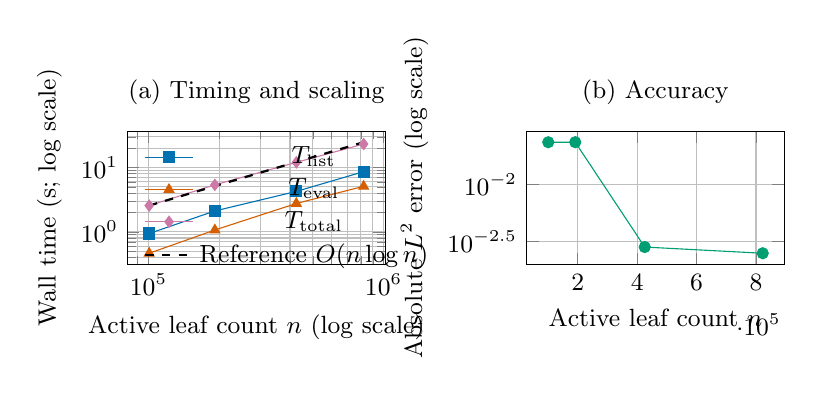
\begin{tikzpicture}
\begin{groupplot}[
  group style={group size=2 by 1, horizontal sep=1.8cm},
  width=0.40\textwidth,
  height=0.27\textwidth,
  grid=both,
  tick label style={font=\small},
  label style={font=\small},
  title style={font=\small},
  legend style={font=\small, draw=none, fill=none},
  every mark/.append style={mark size=2pt}
]
\nextgroupplot[
  title={(a) Timing and scaling},
  xlabel={Active leaf count \(n\) (log scale)},
  ylabel={Wall time (s; log scale)},
  xmode=log,
  ymode=log,
  log basis x={10},
  legend pos=north west
]
\addplot+[color=nature-blue, mark=square*] coordinates
  {(100656,0.941) (191544,2.110) (425498,4.250) (822720,8.622)};
\addlegendentry{\(T_{\mathrm{list}}\)}
\addplot+[color=nature-red, mark=triangle*] coordinates
  {(100656,0.464) (191544,1.067) (425498,2.761) (822720,5.099)};
\addlegendentry{\(T_{\mathrm{eval}}\)}
\addplot+[color=nature-purple, mark=diamond*] coordinates
  {(100656,2.560) (191544,5.376) (425498,12.027) (822720,23.182)};
\addlegendentry{\(T_{\mathrm{total}}\)}
\addplot+[black, dashed, thick, mark=none] coordinates
  {(100656,2.560) (191544,5.143) (425498,12.175) (822720,24.742)};
\addlegendentry{Reference \(O(n\log n)\)}
\nextgroupplot[
  title={(b) Accuracy},
  xlabel={Active leaf count \(n\)},
  ylabel={Absolute \(L^2\) error (log scale)},
  ymode=log
]
\addplot+[color=nature-green, mark=*] coordinates
  {(100656,2.3685e-2) (191544,2.3689e-2)
   (425498,2.8292e-3) (822720,2.4943e-3)};
\end{groupplot}
\end{tikzpicture}
\caption{Dependence of the interaction-list, potential-evaluation, and
total execution times (left) and the \(L^2\) error (right) on the
number of active leaf elements.  The timing panel uses logarithmic axes,
whereas the error panel uses a linear \(n\)-axis and a logarithmic error
axis.}
\label{fig:experiment_n}
\end{figure}

The error remains close to \(2.37\times10^{-2}\) as the number of leaves
increases from \(100\,656\) to \(191\,544\).  A substantial reduction
appears on the \(425\,498\)-leaf mesh.  Refining further to \(822\,720\)
leaves reduces the error by only another \(11.8\%\).  This non-smooth
behavior reflects the discrete marking and conformity closure of the
adaptive mesh, together with the fact that \(p=2\) and \(P=2\) remain
important error sources.

Over the full range, the leaf count increases by a factor of 8.17,
\(T_{\mathrm{list}}\) by a factor of 9.17, and \(T_{\mathrm{eval}}\) by a
factor of 11.0, while \(T_{\mathrm{total}}\) increases by a factor of
9.06.  The \(O(n\log n)\) model established in
Section~\ref{sec:complexity_accuracy} predicts the
factor
\[
\frac{822\,720\log(822\,720)}
     {100\,656\log(100\,656)}
=9.66,
\]
which is close to the measured timing factors.  The dashed reference line
in Fig.~\ref{fig:experiment_n} is normalized to the first
\(T_{\mathrm{total}}\) value.  These results support the intended
\(O(n\log n)\) complexity, although repeated timings over a broader range
of \(n\) are still needed for a formal scaling study.

The importance of balancing the three error mechanisms can be seen from a
separate fine-mesh calculation.  For \(p=6\), \(P=4\),
\(\theta=0.5\), and \(n=822\,720\), the measured values are
\(T_{\mathrm{list}}=8.513\) seconds,
\(T_{\mathrm{eval}}=15.841\) seconds, and
\(T_{\mathrm{total}}=39.235\) seconds, with
\(E_{L^2}=2.0149\times10^{-4}\).  Compared with the corresponding
\(100\,656\)-leaf result, the eightfold mesh increase reduces the error by
only \(8.3\%\), showing that mesh refinement is no longer the dominant
error-reduction mechanism for this parameter combination.

\subsection{Comparison with a uniform mesh at comparable resolution}
\label{sec:uniform_adaptive_comparison}

To isolate the benefit of placing elements adaptively, we compare the
adaptive mesh with a globally refined uniform mesh of nearly the same size.
The adaptive calculation starts from global refinement level 2 and then
applies the two indicator-driven refinement stages described above, producing
\(100\,656\) active leaves.  Global refinement level 4 produces
\(98\,304\) uniform tetrahedra.  Both calculations use \(p=6\), \(P=4\),
\(\theta=0.5\), the CPU backend, \(128\) OpenMP threads, and one target at
the barycenter of every active leaf.  Thus, the source quadrature, singular
neighbor integration, Cartesian expansion, MAC, target rule, and error
definition are identical; only the element distribution differs.

Table~\ref{tab:uniform_adaptive_comparison} reports arithmetic means from
three independent runs.  Here \(T_{\mathrm{mom}}\) is the time required to
form and aggregate the Cartesian multipole moments.  It is included in
\(T_{\mathrm{total}}\), together with mesh processing and the other
preparation costs defined above.

\begin{table}[H]
\centering
\small
\caption{Uniform and adaptive meshes at comparable element counts.  The
treecode parameters are fixed at \(p=6\), \(P=4\), and \(\theta=0.5\).}
\label{tab:uniform_adaptive_comparison}
\begin{tabular}{lrrrrrrrr}
\toprule
Mesh & \(n\) & \(T_{\mathrm{list}}\) &
\(T_{\mathrm{mom}}\) & \(T_{\mathrm{eval}}\) &
\(T_{\mathrm{total}}\) &
\(\|V_{\mathrm{ex}}\|_{L^2,h}\) &
\(E_{L^2}\) & \(E_{L^2}^{\mathrm{rel}}\)\\
\midrule
Adaptive &
\(100\,656\) & 1.008 & 0.142 & 1.478 & 4.534 &
0.134405 & \(2.2434\times10^{-4}\) & \(1.6692\times10^{-3}\)\\
Uniform &
\(98\,304\) & 0.914 & 0.159 & 1.420 & 4.598 &
0.111790 & \(6.0187\times10^{-3}\) & \(5.3839\times10^{-2}\)\\
\bottomrule
\end{tabular}
\end{table}

The total costs are essentially the same: the uniform-to-adaptive
\(T_{\mathrm{total}}\) ratio is \(1.014\).  The uniform calculation has a
slightly lower list and evaluation cost, whereas its global-refinement and
remaining setup costs lead to a slightly larger total time.  At this
comparable cost and element count, the reported adaptive-mesh error is
\(26.8\) times smaller.  This confirms that concentrating elements in the
localized high-variation region is substantially more effective than
distributing approximately the same number of elements uniformly.

The accuracy comparison must nevertheless be interpreted together with the
target quadrature.  For the present Gaussian, the effectively untruncated
analytic norm is \(\|V_{\mathrm{ex}}\|_{L^2}\approx0.134321\).  The adaptive
leaf-barycenter rule gives \(0.134405\), a relative difference of about
\(0.062\%\), while the uniform rule gives \(0.111790\), approximately
\(16.8\%\) below the analytic value.  Hence the uniform level-4 target rule
does not fully resolve the narrow Gaussian peak.  The factor \(26.8\) should
therefore be understood as a production-grid, leaf-barycenter comparison,
rather than as an independent common-grid continuum-error ratio.  A final
mesh-independent verification should evaluate both solutions using the same
higher-order validation rule.


\subsection{Quadrature resolution and integration error}

We first vary \(p\) while fixing \(P=4\), \(\theta=0.5\), and
\(n=100\,656\).

\begin{table}[H]
\centering
\caption{Dependence on the local quadrature accuracy \(p\).}
\label{tab:experiment_p_compact}
\begin{tabular}{rrrrr}
\toprule
\(p\) & \(T_{\mathrm{list}}\) (s) & \(T_{\mathrm{eval}}\) (s) &
\(T_{\mathrm{total}}\) (s) & \(E_{L^2}\)\\
\midrule
2  & 1.063 & 1.060  & 3.484  & \(2.3586\times10^{-2}\)\\
4  & 1.065 & 1.188  & 3.875  & \(1.2143\times10^{-3}\)\\
6  & 1.130 & 1.475  & 4.638  & \(2.1968\times10^{-4}\)\\
8  & 1.111 & 2.016  & 5.775  & \(1.6993\times10^{-4}\)\\
12 & 1.131 & 9.043  & 14.026 & \(1.6020\times10^{-4}\)\\
16 & 1.108 & 29.195 & 35.463 & \(1.5994\times10^{-4}\)\\
\bottomrule
\end{tabular}
\end{table}

\begin{figure}[H]
\centering
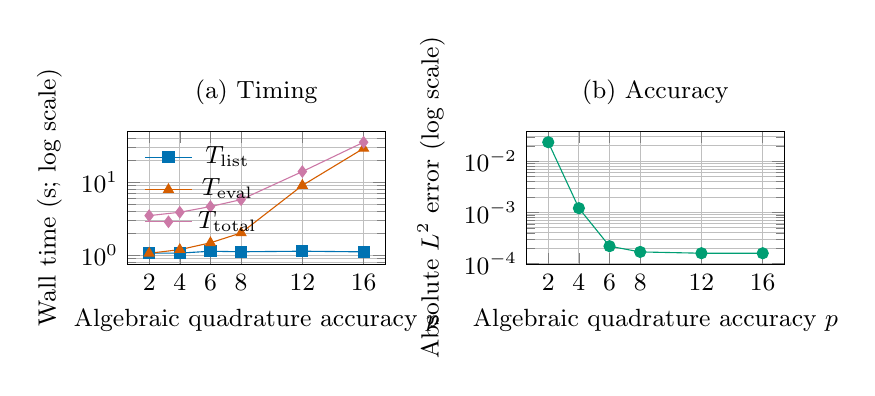
\begin{tikzpicture}
\begin{groupplot}[
  group style={group size=2 by 1, horizontal sep=1.8cm},
  width=0.40\textwidth,
  height=0.27\textwidth,
  grid=both,
  tick label style={font=\small},
  label style={font=\small},
  title style={font=\small},
  legend style={font=\small, draw=none, fill=none},
  every mark/.append style={mark size=2pt}
]
\nextgroupplot[
  title={(a) Timing},
  xlabel={Algebraic quadrature accuracy \(p\)},
  ylabel={Wall time (s; log scale)},
  ymode=log,
  xtick={2,4,6,8,12,16},
  legend pos=north west
]
\addplot+[color=nature-blue, mark=square*] coordinates
  {(2,1.063) (4,1.065) (6,1.130) (8,1.111) (12,1.131) (16,1.108)};
\addlegendentry{\(T_{\mathrm{list}}\)}
\addplot+[color=nature-red, mark=triangle*] coordinates
  {(2,1.060) (4,1.188) (6,1.475) (8,2.016) (12,9.043) (16,29.195)};
\addlegendentry{\(T_{\mathrm{eval}}\)}
\addplot+[color=nature-purple, mark=diamond*] coordinates
  {(2,3.484) (4,3.875) (6,4.638) (8,5.775) (12,14.026) (16,35.463)};
\addlegendentry{\(T_{\mathrm{total}}\)}
\nextgroupplot[
  title={(b) Accuracy},
  xlabel={Algebraic quadrature accuracy \(p\)},
  ylabel={Absolute \(L^2\) error (log scale)},
  ymode=log,
  xtick={2,4,6,8,12,16}
]
\addplot+[color=nature-green, mark=*] coordinates
  {(2,2.3586e-2) (4,1.2143e-3) (6,2.1968e-4)
   (8,1.6993e-4) (12,1.6020e-4) (16,1.5994e-4)};
\end{groupplot}
\end{tikzpicture}
\caption{Effect of the quadrature accuracy \(p\) on the interaction-list,
potential-evaluation, and total execution times (left) and on the
\(L^2\) error (right).  Both ordinates use logarithmic scaling.}
\label{fig:experiment_p}
\end{figure}

Increasing \(p\) from 2 to 4 reduces the error by \(94.9\%\), and the
increase from 4 to 6 gives a further reduction of \(81.9\%\).  The error
then approaches a plateau: increasing \(p\) from 8 to 16 reduces the error
by only \(5.9\%\), whereas \(T_{\mathrm{eval}}\) increases from \(2.016\)
to \(29.195\) seconds.  The nearly constant values of
\(T_{\mathrm{list}}\) are expected because neither the mesh nor the MAC
geometry changes with \(p\).  These data indicate that the near-field
quadrature error dominates at small \(p\), but other error components
become dominant by approximately \(p=6\)--8.

In agreement with the cost model in
Section~\ref{sec:complexity_accuracy},
\(T_{\mathrm{eval}}\) grows by a factor of \(27.5\) and
\(T_{\mathrm{total}}\) by a factor of \(10.2\) from \(p=2\) to 16, while
\(T_{\mathrm{list}}\) remains constant up to measurement noise.

\subsection{Multipole truncation and computational cost}

We next vary \(P\) while fixing \(p=6\), \(\theta=0.5\), and
\(n=100\,656\).  The number of symmetric Cartesian coefficients retained
per cluster is \(N_P=\binom{P+3}{3}\).

\begin{table}[H]
\centering
\caption{Dependence on the Cartesian multipole order \(P\).}
\label{tab:experiment_P_compact}
\begin{tabular}{rrrrr}
\toprule
\(P\) & \(T_{\mathrm{list}}\) (s) & \(T_{\mathrm{eval}}\) (s) &
\(T_{\mathrm{total}}\) (s) & \(E_{L^2}\)\\
\midrule
2  & 0.961 & 0.801  & 3.655  & \(2.1507\times10^{-3}\)\\
4  & 1.059 & 1.499  & 4.565  & \(2.1968\times10^{-4}\)\\
6  & 1.011 & 2.765  & 5.867  & \(1.5126\times10^{-4}\)\\
8  & 1.059 & 5.136  & 8.474  & \(1.4992\times10^{-4}\)\\
12 & 1.096 & 15.326 & 19.119 & \(1.4988\times10^{-4}\)\\
16 & 1.030 & 45.853 & 50.240 & \(1.4988\times10^{-4}\)\\
\bottomrule
\end{tabular}
\end{table}

\begin{figure}[H]
\centering
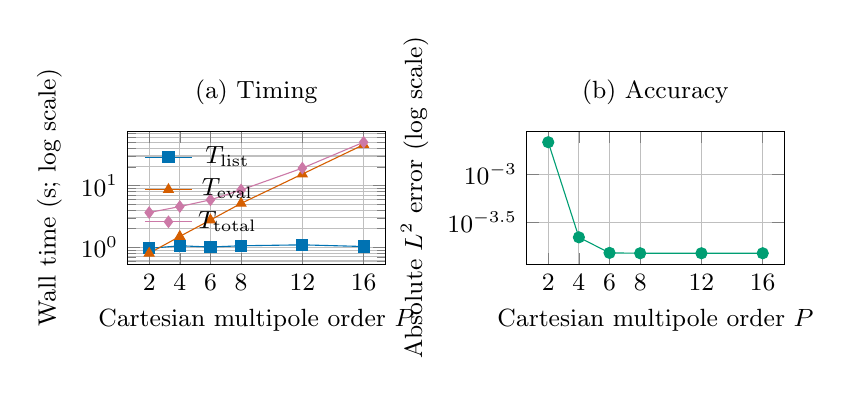
\begin{tikzpicture}
\begin{groupplot}[
  group style={group size=2 by 1, horizontal sep=1.8cm},
  width=0.40\textwidth,
  height=0.27\textwidth,
  grid=both,
  tick label style={font=\small},
  label style={font=\small},
  title style={font=\small},
  legend style={font=\small, draw=none, fill=none},
  every mark/.append style={mark size=2pt}
]
\nextgroupplot[
  title={(a) Timing},
  xlabel={Cartesian multipole order \(P\)},
  ylabel={Wall time (s; log scale)},
  ymode=log,
  xtick={2,4,6,8,12,16},
  legend pos=north west
]
\addplot+[color=nature-blue, mark=square*] coordinates
  {(2,0.961) (4,1.059) (6,1.011) (8,1.059) (12,1.096) (16,1.030)};
\addlegendentry{\(T_{\mathrm{list}}\)}
\addplot+[color=nature-red, mark=triangle*] coordinates
  {(2,0.801) (4,1.499) (6,2.765) (8,5.136) (12,15.326) (16,45.853)};
\addlegendentry{\(T_{\mathrm{eval}}\)}
\addplot+[color=nature-purple, mark=diamond*] coordinates
  {(2,3.655) (4,4.565) (6,5.867) (8,8.474) (12,19.119) (16,50.240)};
\addlegendentry{\(T_{\mathrm{total}}\)}
\nextgroupplot[
  title={(b) Accuracy},
  xlabel={Cartesian multipole order \(P\)},
  ylabel={Absolute \(L^2\) error (log scale)},
  ymode=log,
  xtick={2,4,6,8,12,16}
]
\addplot+[color=nature-green, mark=*] coordinates
  {(2,2.1507e-3) (4,2.1968e-4) (6,1.5126e-4)
   (8,1.4992e-4) (12,1.4988e-4) (16,1.4988e-4)};
\end{groupplot}
\end{tikzpicture}
\caption{Effect of the multipole order \(P\) on the interaction-list,
potential-evaluation, and total execution times (left) and on the
\(L^2\) error (right).  Both ordinates use logarithmic scaling.}
\label{fig:experiment_P}
\end{figure}

Increasing \(P\) from 2 to 4 reduces the error by \(89.8\%\), while the
increase from 4 to 6 yields a further reduction of \(31.1\%\).  For
\(P\geq8\), the error is essentially unchanged at
\(1.499\times10^{-4}\).  In contrast, \(T_{\mathrm{eval}}\) grows from
\(2.765\) seconds at \(P=6\) to \(45.853\) seconds at \(P=16\), consistent
with the rapid growth of \(N_P\).  Thus \(P=4\) provides a favorable
time--accuracy balance, while \(P=6\) is useful when accuracy close to the
observed error floor is required.  The plateau is associated with the
complete discretization error and does not imply that the isolated
multipole expansion fails to converge.

As predicted by the coefficient count in
Section~\ref{sec:complexity_accuracy}, the observed
\(T_{\mathrm{eval}}\) increases by a factor of \(57.2\), from \(0.801\)
to \(45.853\) seconds, and \(T_{\mathrm{total}}\) increases by a factor
of \(13.7\).

\subsection{Sensitivity to the multipole acceptance criterion}

We vary \(\theta\) while fixing \(p=6\), \(P=4\), and \(n=100\,656\).

\begin{table}[H]
\centering
\caption{Sensitivity to the MAC parameter \(\theta\).}
\label{tab:experiment_theta_compact}
\begin{tabular}{rrrrr}
\toprule
\(\theta\) & \(T_{\mathrm{list}}\) (s) & \(T_{\mathrm{eval}}\) (s) &
\(T_{\mathrm{total}}\) (s) & \(E_{L^2}\)\\
\midrule
0.1 & 7.337 & 86.288 & 94.906 & \(1.4988\times10^{-4}\)\\
0.3 & 1.137 & 4.692  & 7.688  & \(1.5033\times10^{-4}\)\\
0.5 & 1.107 & 1.481  & 4.527  & \(2.1968\times10^{-4}\)\\
0.7 & 0.945 & 0.756  & 3.819  & \(7.8256\times10^{-4}\)\\
0.9 & 0.619 & 0.482  & 3.222  & \(2.8872\times10^{-3}\)\\
\bottomrule
\end{tabular}
\end{table}

\begin{figure}[H]
\centering
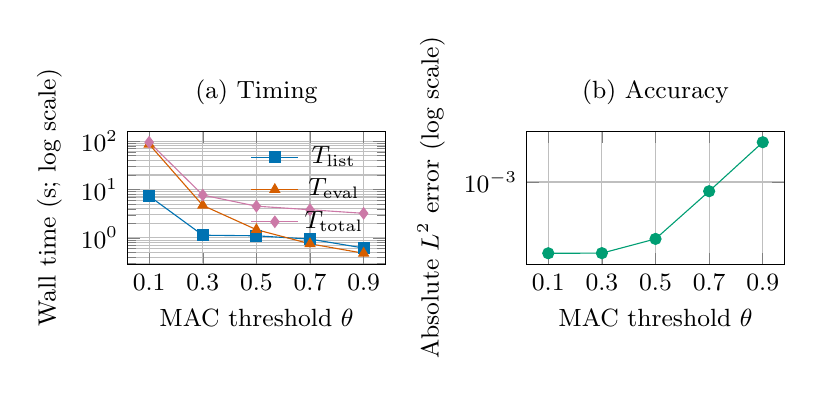
\begin{tikzpicture}
\begin{groupplot}[
  group style={group size=2 by 1, horizontal sep=1.8cm},
  width=0.40\textwidth,
  height=0.27\textwidth,
  grid=both,
  tick label style={font=\small},
  label style={font=\small},
  title style={font=\small},
  legend style={font=\small, draw=none, fill=none},
  every mark/.append style={mark size=2pt}
]
\nextgroupplot[
  title={(a) Timing},
  xlabel={MAC threshold \(\theta\)},
  ylabel={Wall time (s; log scale)},
  ymode=log,
  xtick={0.1,0.3,0.5,0.7,0.9},
  legend pos=north east
]
\addplot+[color=nature-blue, mark=square*] coordinates
  {(0.1,7.337) (0.3,1.137) (0.5,1.107) (0.7,0.945) (0.9,0.619)};
\addlegendentry{\(T_{\mathrm{list}}\)}
\addplot+[color=nature-red, mark=triangle*] coordinates
  {(0.1,86.288) (0.3,4.692) (0.5,1.481) (0.7,0.756) (0.9,0.482)};
\addlegendentry{\(T_{\mathrm{eval}}\)}
\addplot+[color=nature-purple, mark=diamond*] coordinates
  {(0.1,94.906) (0.3,7.688) (0.5,4.527) (0.7,3.819) (0.9,3.222)};
\addlegendentry{\(T_{\mathrm{total}}\)}
\nextgroupplot[
  title={(b) Accuracy},
  xlabel={MAC threshold \(\theta\)},
  ylabel={Absolute \(L^2\) error (log scale)},
  ymode=log,
  xtick={0.1,0.3,0.5,0.7,0.9}
]
\addplot+[color=nature-green, mark=*] coordinates
  {(0.1,1.4988e-4) (0.3,1.5033e-4) (0.5,2.1968e-4)
   (0.7,7.8256e-4) (0.9,2.8872e-3)};
\end{groupplot}
\end{tikzpicture}
\caption{Effect of the MAC parameter \(\theta\) on the interaction-list,
potential-evaluation, and total execution times (left) and on the
\(L^2\) error (right).  Both ordinates use logarithmic scaling.}
\label{fig:experiment_theta}
\end{figure}

A smaller \(\theta\) imposes a stricter acceptance test and increases both
the list-construction and potential-evaluation costs.  Reducing \(\theta\)
from 0.5 to 0.3 lowers the error from \(2.20\times10^{-4}\) to
\(1.50\times10^{-4}\), but increases \(T_{\mathrm{eval}}\) by a factor of
3.17.  Reducing \(\theta\) further to 0.1 produces no meaningful accuracy
gain and makes the evaluation 18.4 times slower than at \(\theta=0.3\).
Conversely, \(\theta=0.7\) and 0.9 are faster but introduce noticeably
larger far-field errors.  The value \(\theta=0.5\) therefore gives a useful
general balance for this test.

Across the tested range,
\(T_{\mathrm{eval}}\) decreases by a factor of \(179\) and
\(T_{\mathrm{total}}\) by a factor of \(29.5\) as \(\theta\) increases
from 0.1 to 0.9, but the error becomes \(19.3\) times larger.  This is the
principal accuracy--cost trade-off controlled by the MAC.

\subsection{ H$_2$O model on a single adaptive mesh}
\label{sec:h2o_single_mesh_experiment}

To test the extension of the adaptive-mesh treecode from a single localized
source to a multicenter geometry, we consider a manufactured H$_2$O problem
on the same truncated domain \(\Omega=[-5,5]^3\).  The three centers, in
Bohr, are
\[
\mathbf R_{\mathrm O}=(0,0,0),\qquad
\mathbf R_{\mathrm H_1}=(1.43043,0,1.10716),\qquad
\mathbf R_{\mathrm H_2}=(-1.43043,0,1.10716).
\]
For each \(A\in\{\mathrm O,\mathrm H_1,\mathrm H_2\}\), define
\[
u_A(\mathbf x)=
\exp\!\left[-4\pi(x-X_A)^2-8\pi(y-Y_A)^2
-12\pi(z-Z_A)^2\right],
\qquad
f_A=-\frac{1}{4\pi}\Delta u_A.
\]
The total source and analytic reference potential are
\[
f(\mathbf x)=\sum_A f_A(\mathbf x),
\qquad
u_{\mathrm{ex}}(\mathbf x)=\sum_Au_A(\mathbf x).
\]
Thus, the example introduces three separated regions of rapid spatial
variation while retaining an exact solution for error measurement.

A single tetrahedral mesh covering the complete cube is refined
simultaneously around all three centers.  The refinement indicator is
\[
I_{\mathrm{all}}(\mathbf x)
=\max_{A\in\{\mathrm O,\mathrm H_1,\mathrm H_2\}}
\frac{1}{|\mathbf x-\mathbf R_A|}.
\]
The total source \(f\) is integrated once on this mesh.  The same hierarchy,
geometric neighborhood construction, MAC, direct near-field quadrature, and
Cartesian far-field expansion used in the single-Gaussian experiments are
then applied without modification.  Only this single-mesh formulation is
considered below.

\begin{figure}[H]
\centering
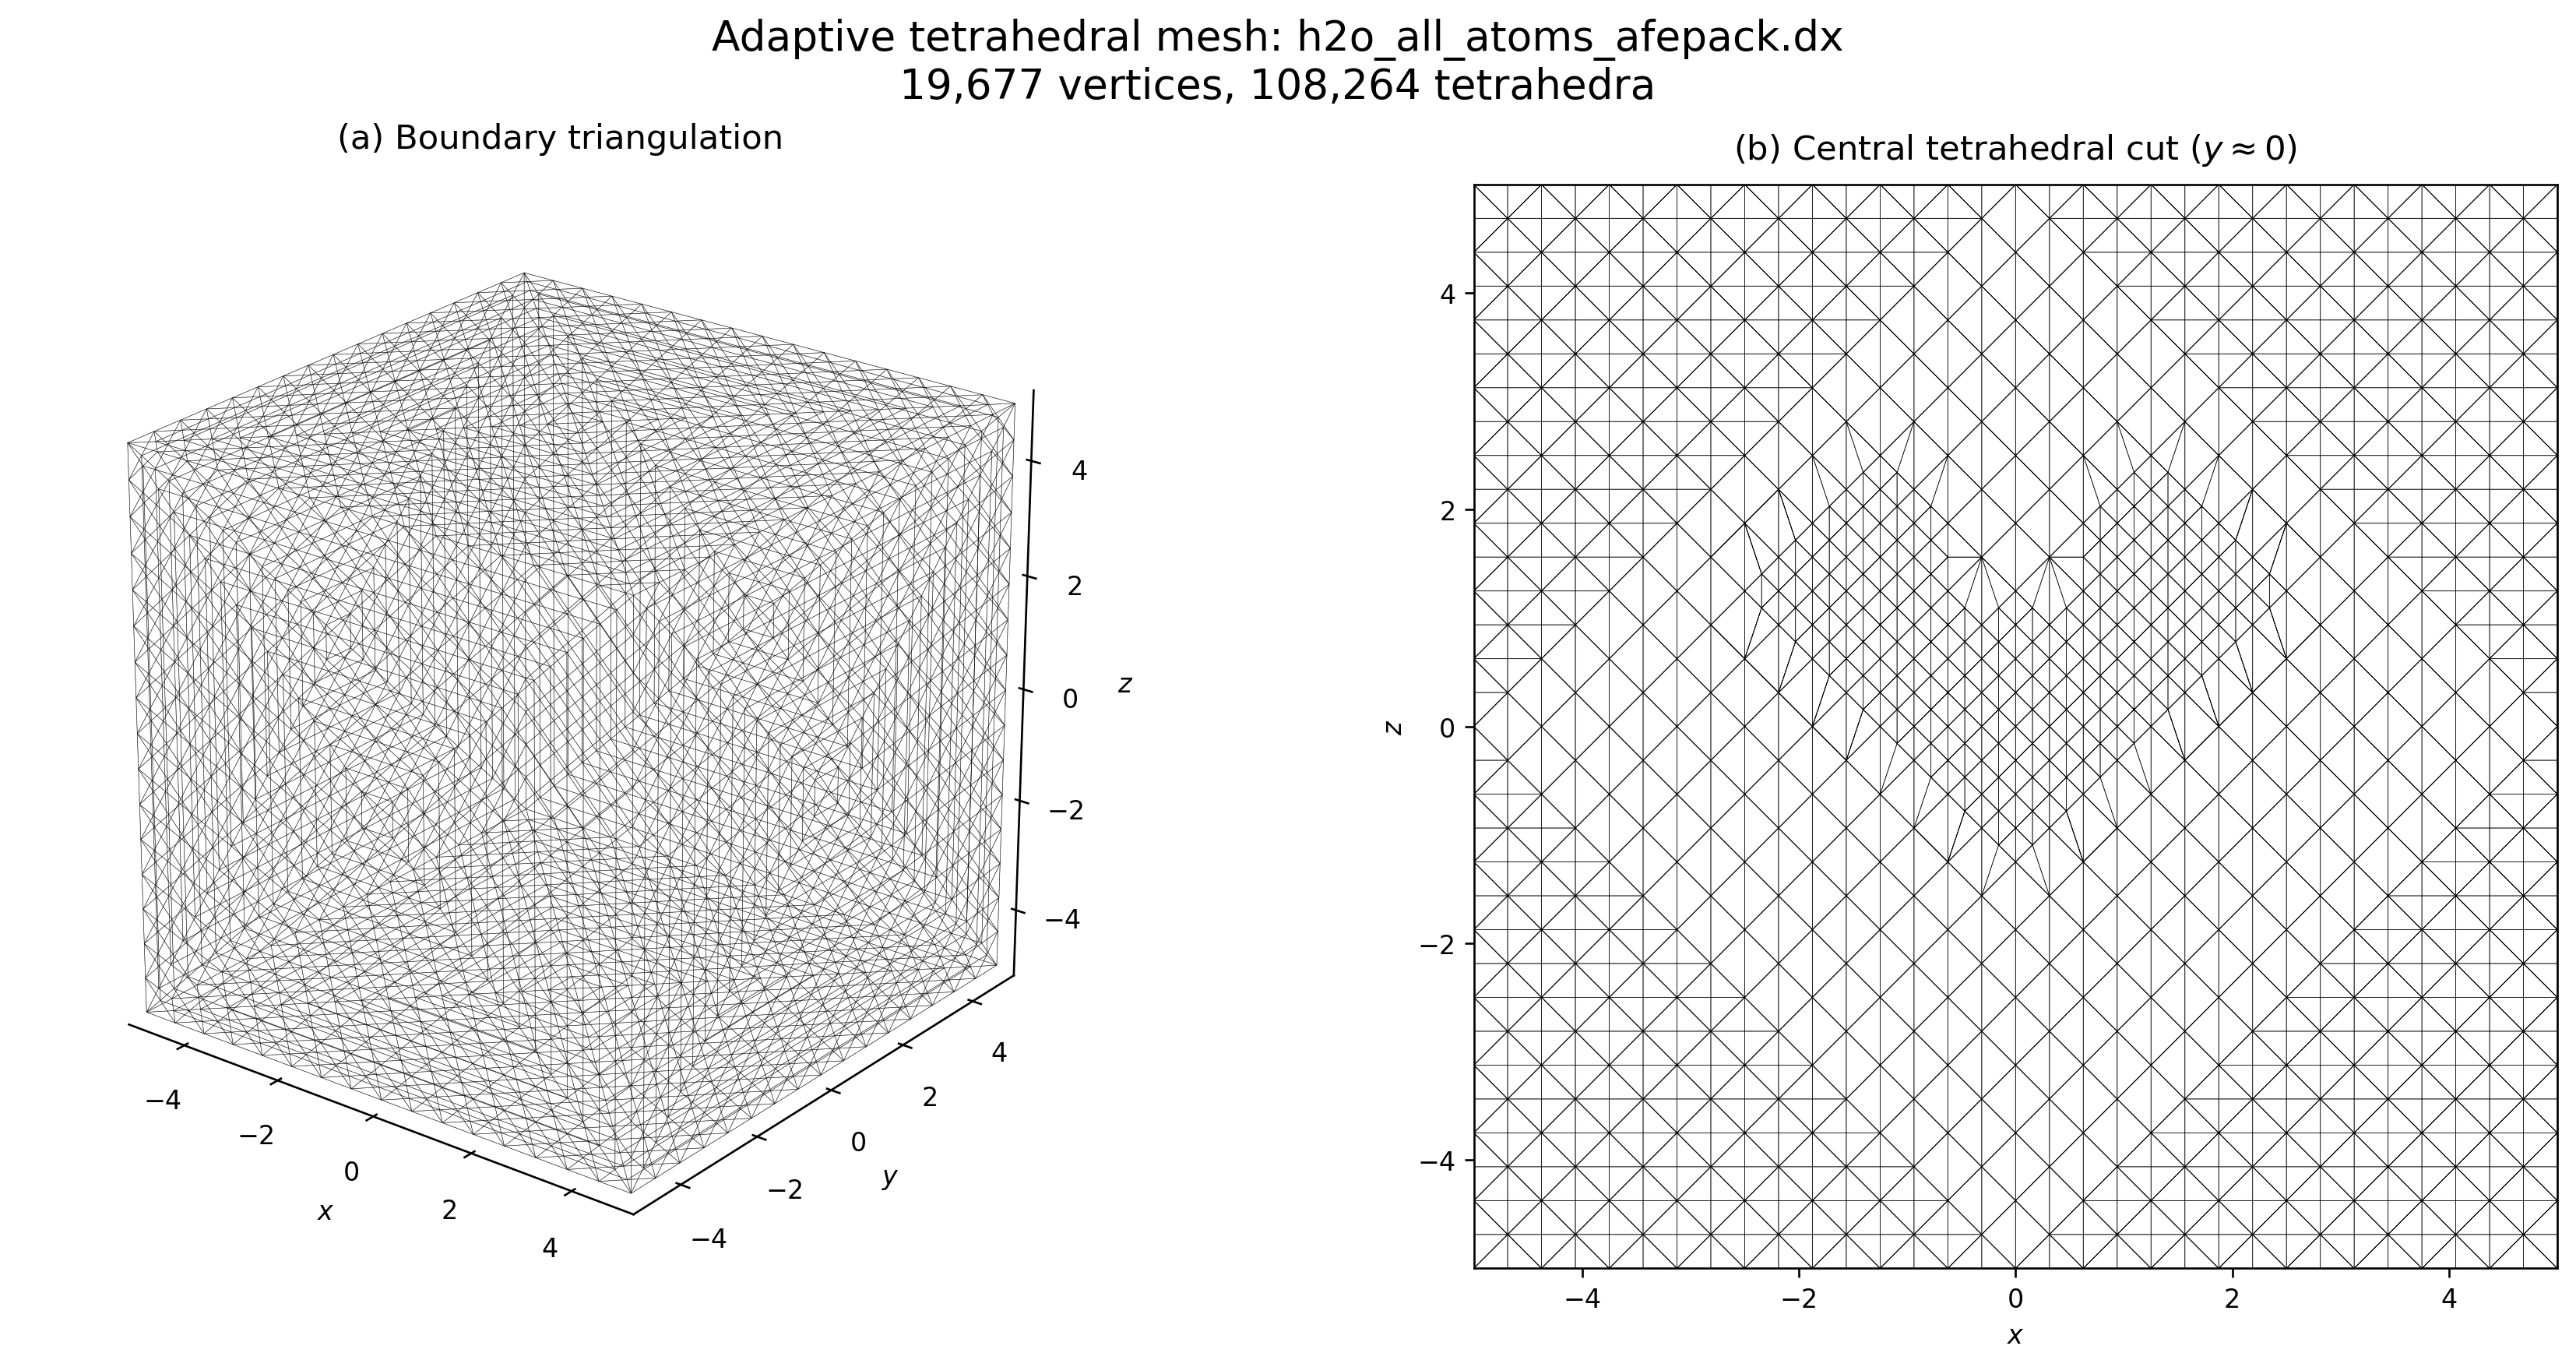
\includegraphics[width=0.96\textwidth]{h2o_all_atoms_tetra_mesh_lines.png}
\caption{Single adaptive tetrahedral mesh refined simultaneously around the
O, H$_1$, and H$_2$ centers.  The boundary triangulation is shown on the
left, and the central cut \(y\approx0\) is shown on the right.  The
regularized mesh contains \(106\,116\) leaf macroelements, corresponding to
\(108\,264\) tetrahedra after decomposition of the twin- and
four-tetrahedron elements.}
\label{fig:h2o_single_all_atom_mesh}
\end{figure}

The calculation uses algebraic quadrature accuracy \(p=6\), Cartesian
multipole order \(P=4\), MAC threshold \(\theta=0.5\), adaptive tolerance
\(10^{-3}\), and \(128\) OpenMP threads on the CPU.  One potential value is
evaluated at the volume-weighted center of each leaf.  The measured result
is summarized in Table~\ref{tab:h2o_single_mesh_result}.

\begin{table}[H]
\centering
\caption{Single-mesh H$_2$O result for \(p=6\), \(P=4\),
\(\theta=0.5\), and adaptive tolerance \(10^{-3}\).}
\label{tab:h2o_single_mesh_result}
\begin{tabular}{rrrrrrr}
\toprule
\(n\) & \(T_{\mathrm{list}}\) (s) & \(T_{\mathrm{prep}}\) (s) &
\(T_{\mathrm{eval}}\) (s) & \(T_{\mathrm{total}}\) (s) &
\(E_{L^2}\) & \(E_{L^2}^{\mathrm{rel}}\)\\
\midrule
\(106\,116\) & 0.207 & 1.412 & 1.794 & 3.413 &
\(4.0302\times10^{-4}\) & \(1.7513\times10^{-3}\)\\
\bottomrule
\end{tabular}
\end{table}

The corresponding discrete norms are
\(\|u_{\mathrm{ex}}\|_{L^2}=0.23012595\) and
\(\|V_h\|_{L^2}=0.22996297\).  This result shows that the existing
single-mesh treecode can treat a simple multicenter source without changing
the interaction algorithm.  It is a manufactured scalability test rather
than a calculation with a physical H$_2$O electron density.


{\color{red} target, set up, results, description, conclusion, advice}

\section{Conclusion}

In this work, we developed a treecode-based method for the efficient evaluation of the Hartree potential on adaptive finite element meshes. The method combines the hierarchical structure of adaptive mesh refinement with treecode acceleration, allowing the mesh itself to serve as the interaction tree without constructing additional spatial data structures.

A geometry-based preprocessing procedure was introduced to organize mesh elements into layered interaction regions. Using vertex connectivity and refinement hierarchy, neighboring and non-neighboring elements can be identified efficiently. This preprocessing step significantly reduces the number of multipole acceptance checks during the evaluation stage and preserves the theoretical complexity of the treecode algorithm on non-uniform meshes.

Within this framework, near-field interactions are computed accurately through elementwise numerical integration, while far-field interactions are approximated using truncated multipole expansions. An error-based multipole acceptance criterion is incorporated to control the approximation error and improve robustness on strongly graded meshes.

The proposed framework provides a effective approach for accelerating Hartree potential evaluation in real-space electronic structure simulations. Because the algorithm relies only on the hierarchical mesh structure, it can be naturally extended to other long-range interaction problems and to more complex multi-center density distributions. Future work will focus on further improving the parallel scalability of the method and extending the framework to large-scale electronic structure calculations.

{\color{red}verify}

\printbibliography



\end{document}
